\chapter{Anforderungsanalyse}\label{chapter3}

\section{Zielgruppe}
Die Zielgruppe dieses Projekts lässt sich relativ schwer eingrenzen. Es betrifft vor allem Personen mit Interesse in Raumfahrt oder dem Weltraum allgemein. Wichtig ist, das diese Personen keinen Bezug zur Informatik aufweisen müssen und zum Beispiel die Bedienung des User Interface daher kein Spezialwissen erfordern darf. Auch die Visualisierung der Oberfläche muss ohne Vorkenntnisse verständlich sein und dabei trotzdem noch die eigentliche Oberfläche korrekt und realitätsnah repräsentieren. Eine weitere mögliche Zielgruppe sind Schüler und Studenten, welche die Visualisierung unter anderem für Forschungszwecke nutzen können. Das Jet Propulsion Laboratory (JPL), einem Institut der NASA, welches sich auf die Entwicklung von Raumsonden und Satelliten spezialisiert, nutzt intern eine Visualisierung namens Mars Trek (siehe Abschnitt \ref{marsTrek}) bereits um Landeziele für Marsmissionen zu finden und plant dies auch für die Auswahl zukünftiger bemannter Erkundungsmissionen zu nutzen\cite{marsTrek}. Des Weiteren könnte eine Visualisierung in den Forschungsbereichen Astronomie und insbesondere Geologie nützlich sein.

\section{Ist-Zustand}\label{istZustand}
Bevor Anforderungen definiert werden können, müssen alternative Visualisierungen in Betracht gezogen werden. Dieses Projekt soll sich dabei an gängigen Visualisierungen orientieren und versuchen deren Schwächen zu vermindern. Zu beachten ist, dass eine Limitierung auf kostenlose Anwendung vorgenommen, um einen besseren Vergleich für dieses Projekt zu erhalten. Eine bekannte Visualisierung des JPL nennt sich Mars Trek\footnote{https://trek.nasa.gov/mars/index.html} und wurde im Jahr 2015 veröffentlicht. Es ist ein web-basiertes Tool um verschiedene Daten, gesammelt aus unterschiedlichen NASA Missionen, in einer interaktiven 3D Visualisierung zu visualisieren. Eine weitere Visualisierung versteckt sich in der Desktop Version von Google Earth\footnote{https://www.google.com/earth/versions/\#earth-pro}. Google Earth ist wohl einer der populärsten Visualisierungen von Geodaten, insbesondere für die Erde. Und auch wenn es der Name nicht vermuten lässt, befindet sich in der Download-Version seit dem Jahr 2009 auch eine Visualisierung des Mars. Im folgenden werden die Alternativen beschrieben und deren Stärken und Schwächen hervorgehoben.

\subsection{Mars Trek}\label{marsTrek}
Das erste, was bei der Anwendung negativ auffällt, sind die langen Ladezeiten, die noch vor der eigentlichen Visualisierung zu sehen sind. Diese liegen beim ersten Laden der Seite im zweistelligen Sekundenbereich bis zur Sichtbarkeit der Visualisierung und ungefähr doppelt so lang bis zum vollständigen Laden der Seite (siehe Abbildung \ref{marsTrekLoading} für ein durchschnittliches Laden). Nachfolgende Ladezyklen sind dann dank Cachings deutlich schneller, die Ladezeiten sind aber für ein anfangs sehr gering aufgelöstes 2D Bild trotzdem sehr hoch. Zwar sind dadurch anfangs keine visuellen Artefakte zu sehen, diese werden dann beim Bewegen der Kamera jedoch sichtbar, sodass die Nützlichkeit in Frage gestellt werden kann.

\begin{figure}[H]
  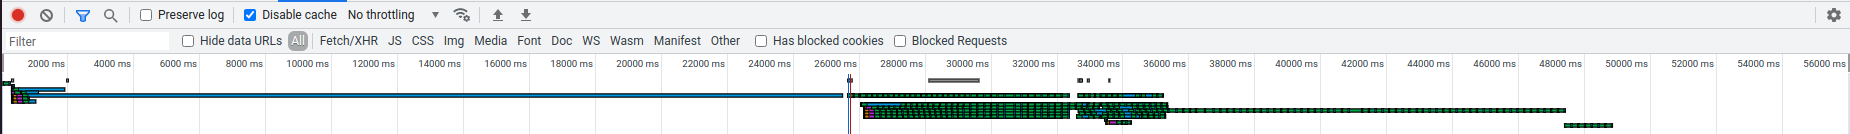
\includegraphics[width=\textwidth,keepaspectratio]{marsTrekLoading.png}
  \caption{Ladezeiten der Mars Trek Anwendung bei 100 Mbit/s auf Mittelklasse-PC}
  \label{marsTrekLoading}
\end{figure}

Initial wird man von der Anwendung mit einer 2D Ansicht des Mars mit Daten der Viking Missionen begrüßt (siehe Abbildung \ref{marsTrekStart}). Zusätzlich wird dem Nutzer ein Tutorial angeboten, was auf eine relativ komplexe Anwendung schließen lässt. Die Anwendung sieht auf den ersten Blick allerdings sehr übersichtlich aus und die einzelnen Menüs lenken nicht von der eigentlichen Visualisierung ab.

\begin{figure}[H]
  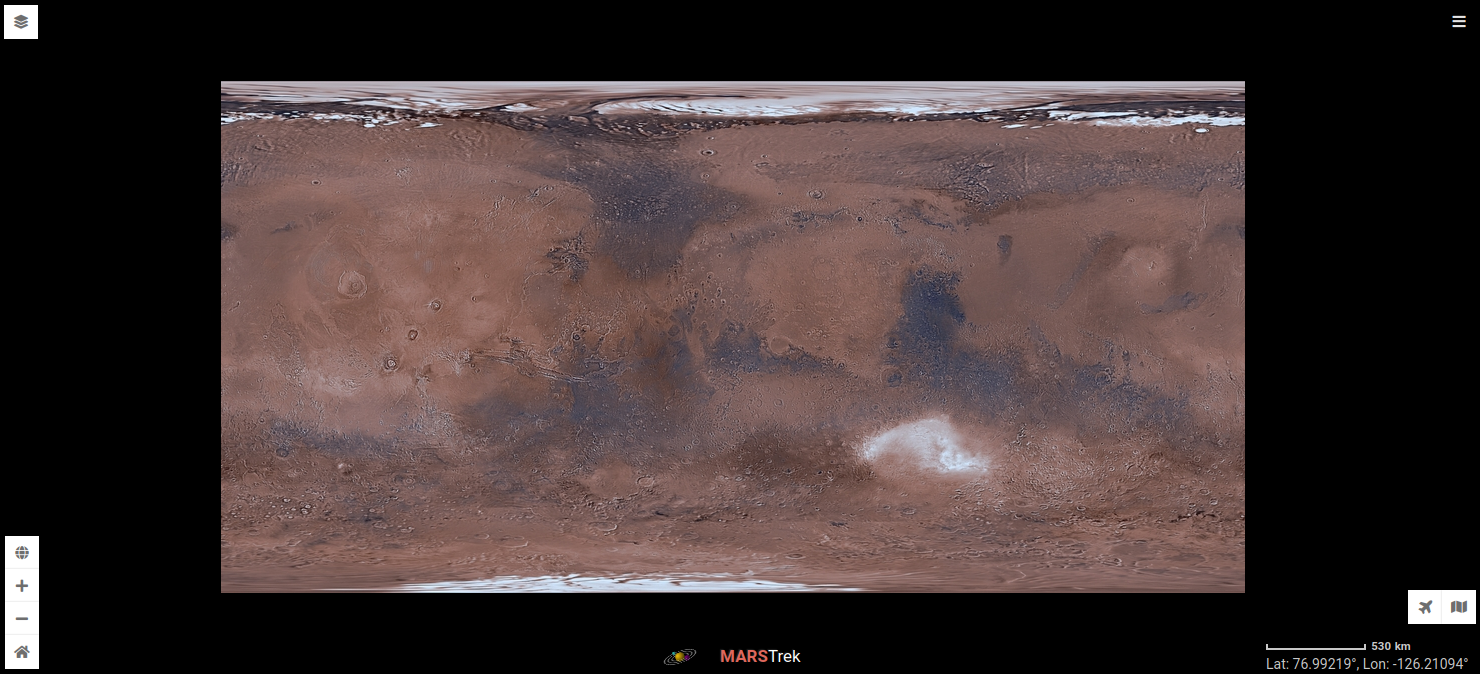
\includegraphics[width=\textwidth,keepaspectratio]{marsTrekStart.png}
  \caption{Initiale Ansicht der Mars Trek Anwendung}
  \label{marsTrekStart}
\end{figure}

Dabei befindet sich in der oberen linken Ecke ein Menü, mit dem man die verwendeten Daten auswählen kann. Unter anderem können auch MOLA Daten gewählt werden, bei denen die Höhenwerte als Farbwerte kodiert sind, ein Punkt, der auch mit diesem Projekt genutzt werden soll. Negativ fällt hier auf, dass die UI hier sehr überladen ist. Es stehen über 2000 verschiedene Datensätze zur Auswahl und die Filter nach Mission, Messinstrument, Koordinaten oder nach verschiedenen (Sub-)Kategorien ist für den Laien schwer verständlich. Auch sind nicht alle Daten für alle Flächen verfügbar, sodass teilweise nicht das gewünschte Resultat zustande kommt und sich verschiedene Ebenen nicht vollständig überlappen. Hier ist zwar ein Zeichentool vorhanden, mit dem man Ausschnitte auf der Karte definieren kann, die als weiterer Filter genutzt werden können, dies ist aber auch nicht intuitiv verständlich. 

In der unteren linken Ecke befindet sich ein Menü, mit dem man unter anderem die Projektion wechseln kann. Hier stehen eine Projektion der beiden Pole, eine globale 2D Ansicht und eine Projektion als Kugel zur Auswahl. Hier könnte das Wechseln noch intuitiver gemacht werden, da die Ansicht als 3D Modell das Highlight der Anwendung sein sollte und die derzeitige Lösung sehr versteckt ist. Des Weiteren lässt sich in dem Menü der Zoom in kleinen Schritten vergrößern und verkleinern, was durch ein Scrollen des Mausrads deutlich leichter fällt. Auch existiert dort ein Button, um die Visualisierung wieder auf den Startzustand zurückzusetzen. Wenn die 3D Ansicht ausgewählt wurde, ist zusätzlich ein Button eingeblendet, mit dem man zwischen einer statischen Kameraansicht und einer frei bewegbaren Kamera wählen kann. Die statische Kamera kann genutzt werden, um in einem festen Abstand um den Planeten zu rotieren und die dynamische Kamera bewegt sich entlang der Blickrichtung und lässt sich durch die bekannten Steuerungstasten WASD oder Pfeiltasten steuern. Dadurch lassen sich bestimmte Orte viel genauer ansteuern, was ein deutlicher Pluspunkt ist.

In der oberen rechten Ecke befindet sich ein allgemeines Menü, in dem verschiedene nützliche Tools vorhanden sind, unter anderem um Distanzen und Höhenprofile zu messen, eine 3D Datei zu erstellen oder die Winkel zur Sonne über die Zeit zu berechnen. Auch diese Tools sind für den durchschnittlichen Nutzer sicherlich nicht besonders nützlich. Auch sind diese Tools nicht in der 3D Ansicht vorhanden, was aus der reinen Machbarkeit keinen Sinn ergibt. Des Weiteren sind hier allgemeine Informationen über die Anwendung, die Entwickler, Release Notes oder Systemanforderungen zu finden. Letzte belegen, dass die Anwendung mit WebGL programmiert wurde und dass die 3D Ansicht einen relativ neuen Browser benötigt.

In der unteren rechten Ecke existiert zum einen eine Möglichkeit, zu bestimmten Koordinaten zu springen. Zum anderen befindet sich dort eine Übersicht, welche den Datensatz auf den einzelnen Ebenen anzeigt. Auch kann hier die Sichtbarkeit einzelner Ebenen angepasst werden, falls diese sich überlappen sollen. Abschließend befindet sich dort eine Skala, die die Längen in Kilometern einer Länge auf dem Bildschirm zuordnet und die Koordinaten des Punktes unter dem Mauszeiger. Hier wird allerdings die Angabe der Höhe vermisst, welche sich wunderbar in das Menü integrieren würde. Generell scheint es keine Möglichkeit zu geben, sich mehr Informationen zu einem bestimmten Punkt anzeigen zu lassen, was für bestimmte geografische Features durchaus sinnvoll sein könnte.

Alles in allem ist die Anwendung ein sehr gutes Beispiel und das generelle Design und viele Features können übernommen werden. Allerdings soll gerade im Hinblick auf eine breitere Zielgruppe die Komplexität verringert werden, indem einige Features bewusst nicht übernommen werden. Auch sollte die User Experience (UX) in einigen Menüs überdacht werden. Idealerweise sollte auch auf die langen Ladezeiten verzichtet werden.

\subsection{Google Earth}
Ein Negativpunkt bei dieser Anwendung ist die Tatsache, dass die Web-Version eine Visualisierung des Mars nicht unterstützt. Ein Download ist immer ein weiterer Schritt, den viele Nutzer, welche schnell eine Visualisierung betrachten möchten, nicht unbedingt gehen möchten. Auch hier sollte das Web die technischen Möglichkeiten geben, alle existierenden Features umzusetzen. Und auch bei dieser Anwendung wird man als erstes mit einem sehr textlastigem Tutorial und anschließend von einer sehr umfangreichen Anwendung, mit Blick auf die Erde, begrüßt (siehe Abbilding \ref{googleEarthStart}).

\begin{figure}[H]
  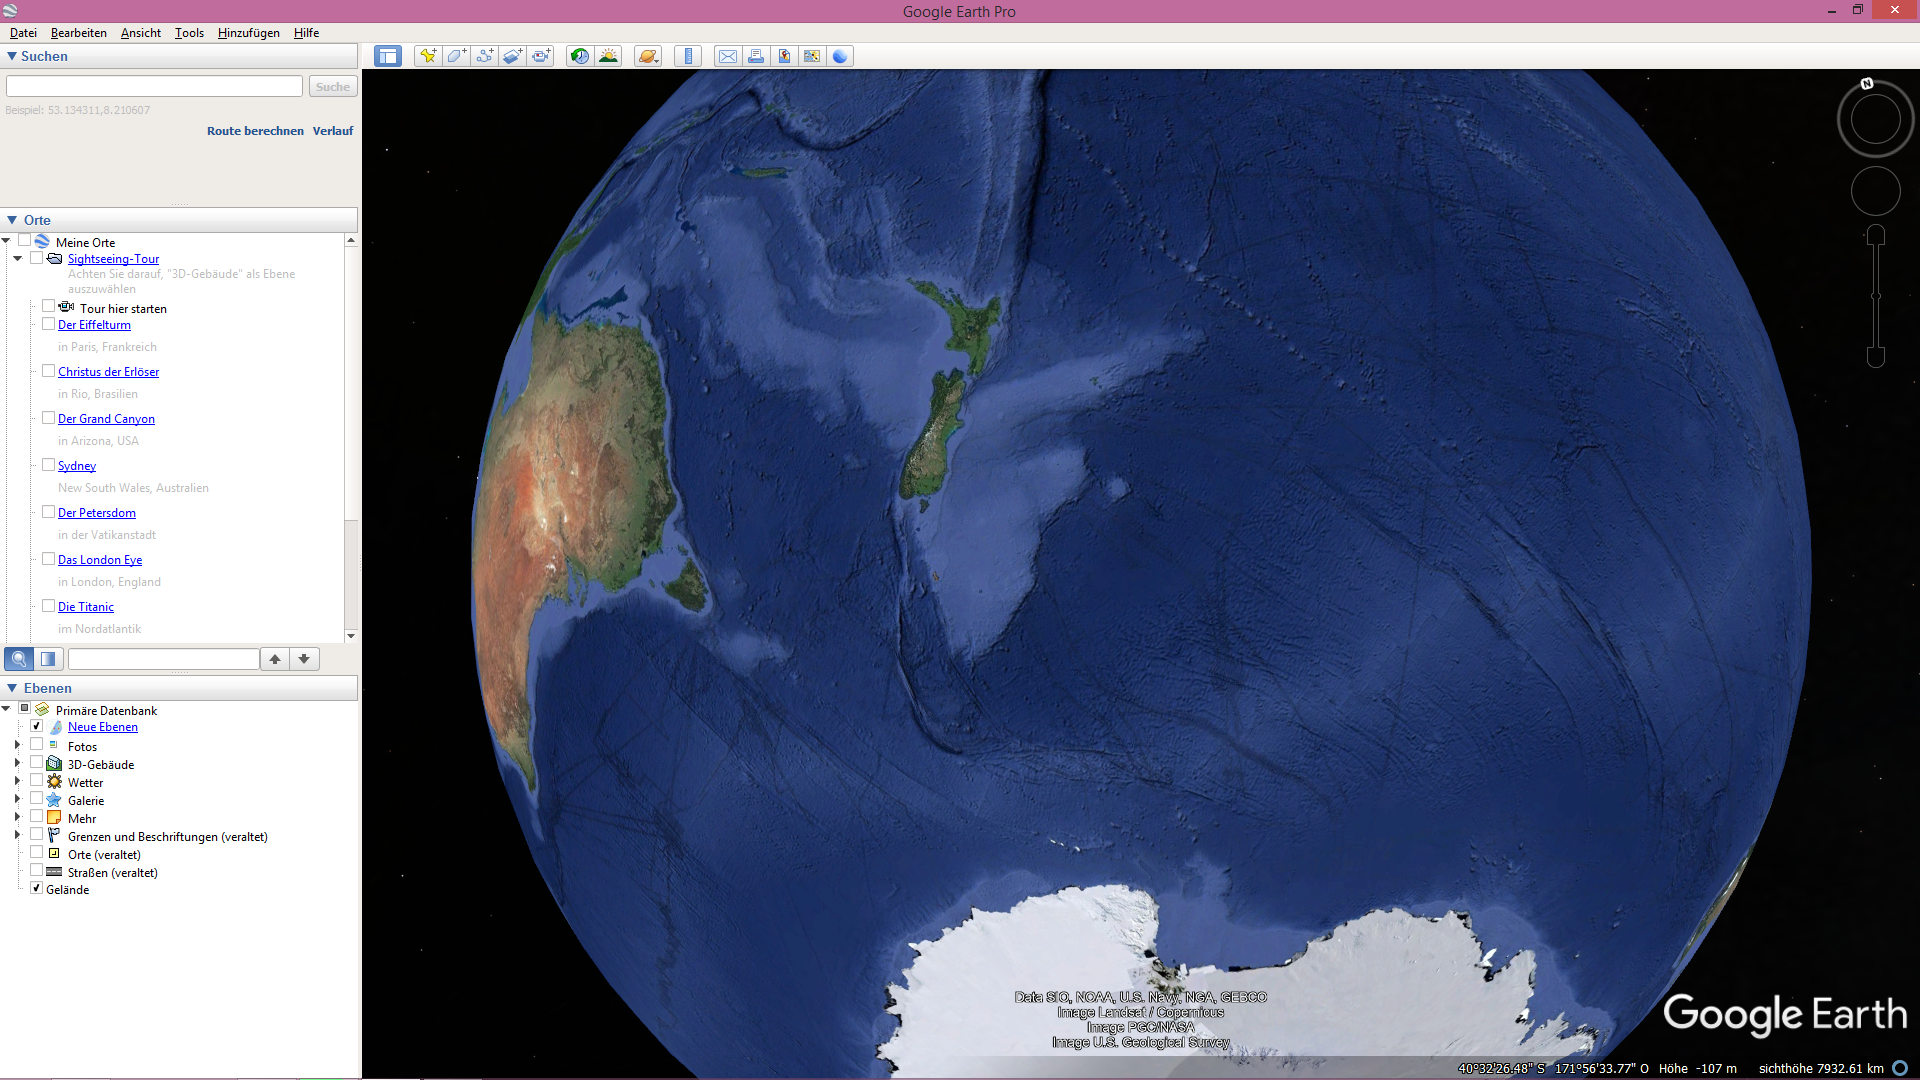
\includegraphics[width=\textwidth,keepaspectratio]{googleEarthStart.png}
  \caption{Initiale Ansicht der Google Earth Anwendung}
  \label{googleEarthStart}
\end{figure}

Hier ist nicht auf Anhieb ersichtlich, wie man die Visualisierung auf den Mars umstellen kann. Es befindet sich die Standard-Windows Menüleiste in der oberen linken Ecke, doch dort sind die Optionen sehr begrenzt. Zusätzlich befindet sich darunter eine weitere Menüleiste, die einige Funktionen aus der eigentlichen Menüleiste besonders dupliziert und so besonders hervorhebt. In den Menüs befinden sich unter anderem verschiedene Tools wie Entfernungsmesser, GPS oder auch ein Flugsimulator, mit dem man die Oberfläche in sehr kreativer Weise erkunden kann. Dies ist ein großer Pluspunkt, allerdings können die wenigsten ein Flugzeug intuitiv steuern und natürlich überschreitet dies den geplanten Projektrahmen bei weitem. Des Weiterem können verschiedene Elemente in der Visualisierung an- und ausgeschaltet werden, unter anderem ein realistische Beleuchtung per Sonne zu verschiedenen Tageszeiten. Auch eine realistische Wasseroberfläche und Atmosphäre, zusammen mit dem realgetreuen Sternenhimmel im Hintergrund, verstärken den Realitätsgrad in sehr großer Weise. Des Weiteren sind Ansichten wie ein Gitternetz mit Breiten- und Längenangaben und eine Minimap in der Ecke sehr hilfreich bei der Navigation. Weitere Menüpunkte dienen zum Wechseln zwischen Google Maps oder der Web-Version. Ein Wechsel von einer Download-Version zum Browser ist hierbei fragwürdig, vor allem da alle Funktionen der Web-Version auch in dieser Version vorhanden sind. Ein etwas kurioses Problem verbirgt sich hinter dem Menüpunkt ''Regionating durchführen''. Zum einen ist nicht verständlich, was man mit dem sich öffnenden Fenster verwirklichen kann, zum anderen lässt sich dieses Fenster einfach nicht mehr schließen, da die entsprechenden Buttons deaktiviert wurden. Warum so ein Usability-Problem bei einer so bekannten Anwendung einer so bekannten Firma beim Testen nicht entdeckt wurde ist nicht verständlich.

Schlussendlich findet man den Button zum Wechseln des Planeten unter den Menüpunkten ''Ansicht'' und dann ''Erkunden'', eine Wahl, die auf den ersten Blick nicht verständlich erscheint. Sobald man es geschafft hat, die Anwendung auf die Mars Visualisierung umzuschalten, fällt auf, dass gar keine 3D Höhendaten angezeigt werden, sondern Kamerabilder verschiedenster Marsmissionen als Textur auf eine Kugel projiziert wurden. Hierbei fällt auf, dass nicht immer die gleichen Daten für alle Flächen vorhanden sind und so ein Mix aus verschiedenen Datenquellen genutzt wird. Dies führt zu einem etwas schlechterem visuellen Eindruck (siehe Abbildung \ref{googleEarthMars}).

\begin{figure}[H]
  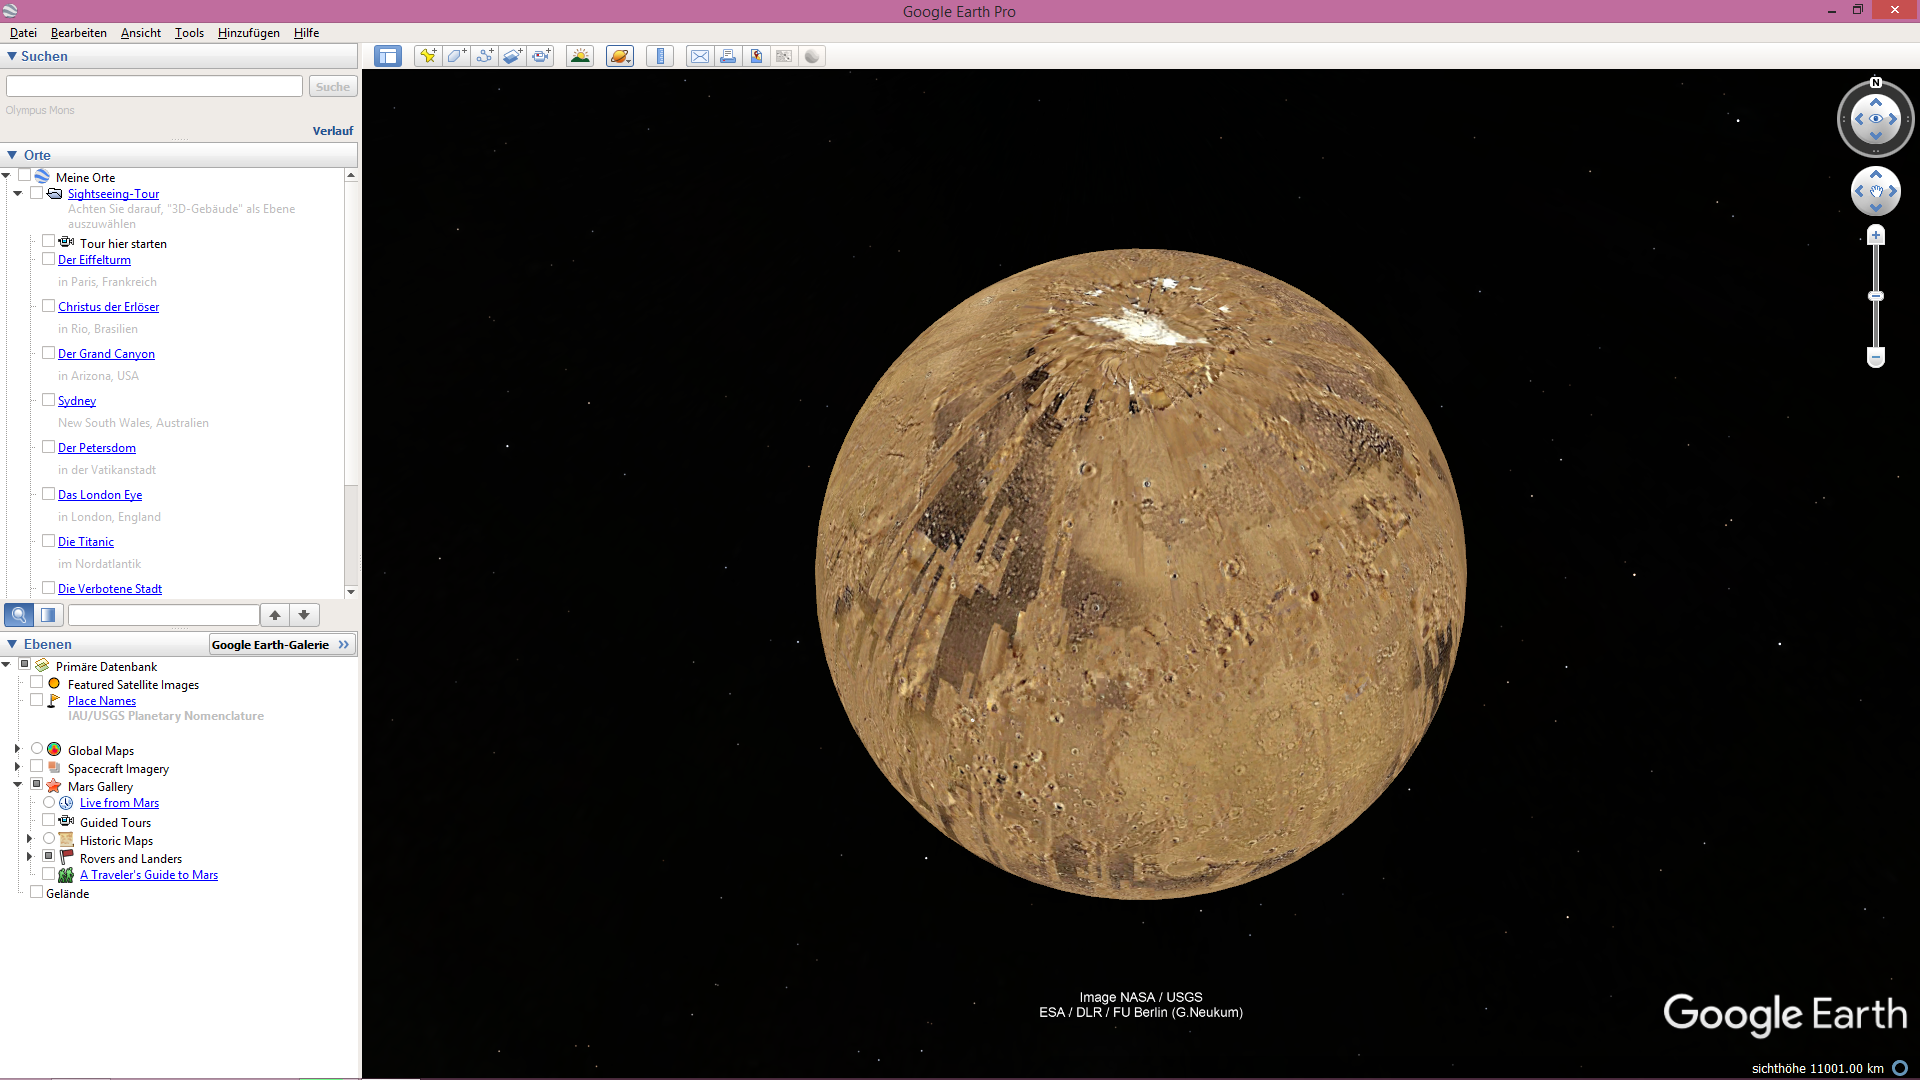
\includegraphics[width=\textwidth,keepaspectratio]{googleEarthMars.png}
  \caption{Initiale Mars Visualisierung der Google Earth Anwendung}
  \label{googleEarthMars}
\end{figure}

Auch diese Anwendung nutzt das Konzept von Ebenen um verschiedene Daten auf dem Globus gleichzeitig anzuzeigen. Hier wird der Fokus aber mehr auf verschiedene Dinge gelegt, welche sich in vollständig in die Visualisierung integrieren (z.B. Ortsnamen, Mars Rover oder Fotos bestimmter Marsmissionen). Hier findet man dann auch die Checkbox ''Gelände'', welche eine echte 3D Höhendarstellung ermöglicht. Der wahrscheinlichste Grund, warum dies standardmäßig deaktiviert ist, ist, dass weiterhin Satellietenbilder auf dem Globus angezeigt werden und diese durch eine 3D Darstellung verzerrt werden. Dies verschlechtert die Kantenbildung zwischen benachbarten Satelietenbildern noch weiter. Eine Möglichkeit die Bodendarstellung auf eine weniger realistische Darstellung zu wechseln ist nicht vorhanden. Ein weiteres Problem ist das Panel ''Orte'' auf der linken Seite. Es ist definitiv für die Erde ausgelegt und erlaubt es dem Benutzer zu verschiedenen Sehenswürdigkeiten wie dem Eifelturm oder dem Petersdom zu springen, ein Feature, was auf dem Mars völlig fehl am Platz ist. Immerhin ist die Suchleiste in der oberen linken Ecke funktional und man kann zu bestimmten geographischen Featuren wie dem Olympus Mons springen.

Auf der anderen Seite befindet sich verschiedene Möglichkeiten die Kamera zu bewegen. Zum einen ermöglichen sie die Rotation um den stationären Mars in x- und y-Richtung. Dies ist ebenfalls mit den Pfeiltasten und WASD und durch Ziehen der Maus in eine bestimmte Richtung möglich, was eine deutlich intuitive Steuerung darstellt. Zum anderen ermöglicht es die Rotation des Globus um die z-Achse (Rolling), was nachfolgende Interaktionen sehr verwirrend macht. Eine feste Positionierung des Nordpols nach oben ist eine allgemein bekannte Darstellung (auch bei physischen Globen) und ein Ändern dieser Darstellung sollte den wenigsten Nutzern von Vorteil sein. Des Weiteren ist auch hier eine Möglichkeit gegeben, den Zoom per Mausklick anzupassen. Da dies per Mausrad jedoch deutlich einfacher ist, ist auch hier der Nutzen in Frage gestellt. Eine frei im Raum bewegliche Kamera ist nicht vorhanden (mit Ausnahme des Flugsimulators), sodass bestimmte Orte teilweise recht umständlich erreicht werden können. In der unteren rechten Ecke befinden sich noch die Koordinaten der Position des Mauszeiger auf dem Planeten und eine Angabe, in welcher Höhe sich die Kamera über dem Erdboden befindet. Dies ist eine sehr nützliche Information um Abstände einordnen zu können. Allerdings wird auch hier die Höhenangabe des Punktes auf dem Planeten nicht angezeigt. Auch das übergroßes Logo (15\% der Gesamtbreite) in der Ecke ist etwas ablenkend und hat keinen funktionalen Nutzen.

Alles in allem ist auch diese Anwendung sehr komplex und für Laien nicht als Visualisierung des Mars erkenntlich. Es kommt auch das Gefühl auf, als ob diese Anwendung ursprünglich nicht für die Visualisierung weiterer Planeten gedacht ist, ein Punkt, der wegen des Namens sehr wahrscheinlich scheint. Die Benutzerführung sollte verbessert werden und doppelte Wege ein bestimmtes Ziel aus Nutzersicht zu erreichen vermieden werden. Ein großer Pluspunkt dieser Anwendung ist der unglaublich hohe Realitätsgrad mit hochaufgelösten Bildern bei hohen Zoomfaktoren und den verschiedenen Möglichkeiten Wetter, Sonne, Wasser und ähnliche Dinge physikalisch korrekt in die Visualisierung einfließen zu lassen. Dieser Realitätsgrad wird jedoch durch den Mix aus verschiedenen Satellietenbildern stark gestört.

\section{Anforderungen}
Auf Grund des Prototypen-Charakters dieses Projekts besteht eine geringere Priorisierung bei den funktionalen und nicht-funktionalen Anforderungen. Es sollen möglichst viele verschiedenen Möglichkeiten zur Datenreduzierung (siehe Abschnitt \ref{datenreduzierung} implementiert und evaluiert werden. Die Anwendung soll dennoch einen Nutzen erfüllen um die Evaluation so realistisch wie möglich zu gestalten. Auch hilft dies dabei, die Korrektheit der Implementierungen zu verifizieren, wenn eine vollständige Visualisierung mit verschiedenen Features vorhanden ist. Um die konkreten Anforderungen zu ermitteln, wurden diverse Personen aus der Zielgruppe nach ihren Wünschen befragt. Aus diesen Wünschen wurden die Features priorisiert, die von den meisten Personen gewünscht wurden. Des Weiteren wurden die Stärken der bisher analysierten Visualisierungen in Betracht gezogen und in die Anforderungen integriert. Bestimmte Features, welcher im gegebenem Projektzeitraum nicht umsetzbar waren, wurden dabei im voraus verworfen.

\subsection{Funktional}
Die wichtigste funktionale Anforderung ist eine realistische Darstellung des Mars mit den beschriebenen MOLA Daten. Dabei soll eine reine 3D Darstellung gewählt werden, bei der die Höhenwerte realistisch den Globus verformen, das Anzeigen einer Textur der Oberfläche auf einer 3D Kugel soll nicht genutzt werden. Der Hauptgrund dafür ist die realistischere Darstellung, besonders bei hohen Zoomstufen. Des Weiteren hilft es dabei, die Datenreduzierung besser zu evaluieren, da das Generieren einer Textur aus den Daten eine einmalige Tätigkeit darstellt und auch keinem Zwang der Datenreduzierung unterliegt. Es kann unabhängig von der Laufzeit beliebig lange dauern und die Größe von einzelnen Texturen ist zwar durch die OpenGL Implementation limitiert, sie kann aber leicht in einzelne kleinere Texturen aufgeteilt werden. Die Gesamtdatenmenge ist dabei nicht vergleichbar mit der Datenmenge von Modellen mit individuellen Höhenwerten. Ein nicht repräsentativer Test auf eigener Hardware zeigte, dass ein Aufteilen der Textur in 4 Abschnitte bereits ausreichen würde um sie in höchster Auflösung anzeigen zu können. Und Techniken wie das frustum- oder occlusion-culling, die zur Laufzeit die Datenmenge reduzieren, sind dabei nicht notwendig. Neben der Projektion der Daten in eine Kugelform soll auch die flache Darstellung ermöglicht werden, bei der allerdings dennoch 3D Koordinaten genutzt werden. Dies soll, anders als bei der MarsTrek Anwendung, allerdings nicht der Standard sein und vom Benutzer bewusst ausgewählt werden müssen. Ein möglicher Nutzen von einer flachen Darstellung ist die bessere Einschätzung von Entfernungen und geraden Linien, was auf einer Kugel oft nicht intuitiv ist.

Für die Darstellung der Oberfläche soll eine schematische Darstellung genutzt werden, bei der keine weiteren Datenquellen notwendig sind. Die Wahl fiel dabei auf eine topographische Darstellung, bekannt aus Atlanten, bei der der Farbwert abhängig vom Höhenwert ist. Der Farbwert wird dabei aus einem vordefiniertem Farbbereich linear interpoliert. Der Hauptgrund für diese Wahl ist vor allem der begrenzte Projektzeitraum. Ein Einbinden von weiteren Quellen zur Bestimmung der Oberflächenbeschaffenheit (z.B. Gesteinsart oder Eis) hätte die Komplexität noch weiter erhöht und wurde in diesem Projekt als nicht durchführbar eingestuft. Die verwendete Farbskala muss dem Benutzer auch mitgeteilt werden, eine entsprechende Übersicht welche Farbe zu welchem Höhenwert gehört, muss also angezeigt werden. Dabei sollen die Ränder der Skala vom Benutzer konfigurierbar sein. Der Nutzer soll also effektiv bestimmen können, welcher minimale und maximale Höhenwert für die lineare Interpolation genutzt wird. Welche Farben genutzt werden, muss noch evaluiert werden, der Nutzer soll diese aber nicht ändern können, da dafür kein Use-Case gefunden wurde und es die Komplexität unnötig erhöht. Standardmäßig soll ein minimaler und maximaler Wert gefunden werden, der eine möglichst gleichmäßige Farbverteilung ermöglicht. Besondere Extreme, wie zum Beispiel der Olympus Mons, sollten dabei außen vor gelassen werden, da es die Skala sonst stark in eine Richtung verzerrt und die Farbverteilung so stark verringert.

Für die Interaktion mit dem Mars sollen verschiedene Möglichkeiten genutzt werden, die möglichst intuitiv sind und keiner textuellen Erklärung benötigen. Zum einen betrifft das die Steuerung der Kamera. Dies ist ein wichtiger Aspekt im Design des Prototypen und es muss darauf geachtet werden, dass die Bewegung sowohl aus der Ferne flüssig ist, also auch bei hoher Zoomstufe noch präzise bestimmte Orte betrachtet werden können. Zum einen soll hier eine stationäre Kamera implementiert werden, die in einem festen Abstand um den Globus rotiert. Die Rotation soll dabei mit der Maus erfolgen und auch das Ändern des Abstands, höchstwahrscheinlich mit dem Mausrad, ermöglichen. Zum anderen soll eine frei bewegliche Kamera implementiert werden, die mit der Tastatur frei in alle 6 Richtungen gesteuert werden kann. In dieser Konfiguration soll man sich mit der Maus umschauen können und sich dann entsprechend der Blickrichtung bewegen können. Diese Kamera muss in der flachen Projektion auch erzwungen werden, da hier natürlich eine Rotation um den Globus nicht möglich ist. Eine weitere wichtige Interaktion soll das Erhalten von Informationen zu bestimmten Orten darstellen. Dabei soll der Benutzer auf einen Punkt auf dem Mars klicken können und dann zumindest die Koordinaten und den exakten Höhenwert angezeigt bekommen. Hier sollte idealerweise der Höhenwert in verschiedenen, vom Benutzer konfigurierbaren Einheiten angezeigt werden um die Zielgruppe noch weiter zu erhöhen. Standardmäßig sollen Meter oder Kilometer als Einheit genutzt werden.

Das Anzeigen von weiteren Informationen ist fakultativ, hier könnte man zum Beispiel auf benannte geologischen Features zurückgreifen, welche von der \textit{Working Group for Planetary System Nomenclature} bereitgestellt werden. Diese werden in einer Datenbank bereitgestellt, welche unter anderem deren Position und Durchmesser beinhaltet, sodass eine Integration machbar wäre\footnote{https://planetarynames.wr.usgs.gov/AdvancedSearch}. Weitere fakultative Anforderungen sind Features aus den analysierten Alternativen, die als hilfreich bei der Navigation eingestuft wurden. Hierzu zählt zum Beispiel das Gitternetz mit Längen- und Breitenangaben, sowie die Möglichkeit zu bestimmten Koordinaten zu springen. Auch wenn bei Darstellung der Oberfläche dieser Anwendung nicht realitätsnah werden soll, könnte man den Realitätsgrad dennoch deutlich erhöhen. Besonders die Google Earth Anwendung hat dies in sehr guter Weise gezeigt und Features wie eine korrekte Simulation der Sonne mit Licht- und Schatteneffekten zu bestimmten Tageszeiten oder einen realistischen Sternenhimmel im Hintergrund verstärkten die Immersion stark. Eine weitere fakultative Anforderung ist die Integration weiter Datenquellen. Diese Anwendung soll, wenn möglich, möglichst unabhängig von der Datenquelle sein und eine Integration weiterer Datenquellen, inklusive Auswahl durch den Benutzer, ermöglichen. Gute Alternativen sind hier unter anderem Höhendaten des Mondes (z.B. LOLA mit 8GB Rohdaten) oder der Erde (z.B. SRTM mit über 100Gb Rohdaten). Das Konzept von Ebenen, was in den analysierten Alternativen zum Einsatz kam, soll hier explizit nicht verwendet werden, da es in allen Fällen als zu kompliziert und wenig vorteilhaft eingestuft wurde. Der Nutzer soll immer nur Daten eines einzigen Datensatzes angezeigt bekommen.

\subsection{Nicht-Funktional}\label{nichtFunktional}
Die nicht-funktionalen Anforderungen richten sich hauptsächlich an die Qualität der Visualisierung und die Performance. Hier ist es schwer, die formulierten Wünsche in konkrete Anforderungen umzuwandeln, da hier oft subjektive Dinge eine Rolle spielen. Auch lassen sich bestimmte Dinge wie die Performance einfach nicht in der gewünschten Qualität (z.B. in der Form x Frames Per Second (FPS) auf Hardware y) definieren. Insbesondere die Hardwareanforderungen können dabei auf Grund der Hardwarevielfalt nicht genau definiert werden. Eine Kernaussage ist, dass die Anwendung möglichst immer die höchste Datenauflösung anzeigt, die möglich ist. Wie bereits beschrieben (siehe Abschnitt \ref{datenmenge}) ist ein dauerhaftes Anzeigen der höchstmöglichen Datenauflösung auf normaler Hardware einfach nicht umsetzbar. Daher soll die Auflösung immer genau so hoch gewählt werden, dass eine dauerhafte Framerate von ungefähr 30 FPS erreicht wird. Die Framerate sollte möglichst genau getroffen werden, eine Abweichung darunter schadet der User Experience (UX), eine Abweichung darüber erlaubt eine Verbesserung der Datenauflösung. Hier ist also ein sehr starkes Ringen zwischen Performance und Qualität vorhanden. Der Wert wurde, anstatt der üblichen 60 FPS, nur auf ungefähr 30 FPS festgelegt, da die Visualisierung keine starken Bewegungen und somit keine flüssigen Übergange benötigt. Der Nutzer soll zwar die Kamera bewegen können, allerdings liegt der Fokus dabei immer noch auf der Visualisierung an sich.

Ein weiterer Aspekt ist, dass keine dedizierten Ladezeiten vorhanden sein sollen, in denen die Visualisierung nicht zu sehen ist. Dies wird häufig genutzt, um visuelle Ladeartefakte zu verstecken. Diese können zum Beispiel auftreten, wenn neue Abschnitte geladen werden müssen, nachdem der Benutzer die Kamerasicht verändert hat. Idealerweise soll auch auch ohne Ladezeiten der Nutzer nichts von der Trennung in Abschnitte mitbekommen und immer den Mars als Ganzes sehen. Dies kann zum Beispiel erreicht werden, in dem die Bewegung der Kamera antizipiert wird und Abschnitte, welche als nächstes geladen werden müssten, bereits vorgeladen werden.

Wichtig ist, dass die bisherigen nicht-funktionalen Anforderungen immer abhängig von der Hardware des Nutzer sind, da die Visualisierung auf Client-Seite durchgeführt wird. Es kann also kein einheitliches Performance-Konzept geben, welches für alle Nutzer geeignet ist. Zum einen können natürlich einzelne Parameter im voraus für verschiedene Performance-Klassen per Hand definiert werden. Da dafür allerdings eine umfassende Evaluation auf unterschiedlicher Hardware notwendig ist, ist der Zeitaufwand sehr groß. Eine Alternative ist es, zur Laufzeit bestimmte Parameter an die aktuellen Hardware anzupassen. Ein Problem bei beiden Ansätzen ist auch das Erfassen der aktuellen Hardware an sich. Auch ohne sich bereits auf eine Sprache oder Plattform festgelegt zu haben, gibt es meist keinen einheitlichen Weg diese zur Laufzeit zu erfassen. Natürlich könnte man den Nutzer nach der gewünschten Qualität fragen. Dieser Ansatz wird in der Realität sehr oft durchgeführt, allerdings soll die Zielgruppe kein Spezialwissen benötigen und Kenntnisse über die aktuelle Hardware sind nicht überall vorhanden. Ein Ansatz wäre es sich nicht auf die Hardware an sich zu konzentrieren, sondern zur Laufzeit die Auswirkungen zu messen und sich dementsprechend anzupassen. Man könnte zum Beispiel Parameter wie die Framerate als Indikator nutzen und dann zur Laufzeit auf Schwankungen reagieren. Alles in allem soll dieses Projekt als Prototyp dienen und ein Finetuning aller Parameter würde den Projektrahmen sprengen. Daher sind die bisher beschriebenen Anforderungen fakultativ und eher als ungefähre Richtwerte zu verstehen.

Eine Anforderung, auf die großen Wert gelegt werden soll, ist die Skalierbarkeit der Anwendung. Das Ziel dieses Projekts ist die Evaluation von verschiedenen Methoden zur Datenreduzierung. Dies soll idealerweise nicht von den verwendeten Daten abhängen und muss universell funktionieren. Die gesamte Anwendung, mit Ausnahme von Modulen die spezifische Datenformate interpretieren, muss also mit dieser Anforderung gestaltet werden. Ein Kernaspekt dieser Anforderung ist eine strikte Begrenzung von Arbeitsspeicher (RAM) und Grafikkartenspeicher (VRAM). Diese beiden Performancekriterien sind gut geeignet, die Qualität der Datenreduzierung zu beurteilen. Wichtig ist auch hier, dass der verwendete Datensatz keinen Einfluss auf die Anforderung hat, die gleichen Anforderungen müssen auch für einen Datensatz gelten, der mehrere hunderte Male größer ist. Als konkrete obere Grenze wurde Richtwerte an Mittelklasse Computer verwendet und bestehen aus 8 GB für den RAM und 4 GB für den VRAM. Eine Konsequenz, die sich aus diesen Anforderung ergibt ist, dass die Quelldaten niemals vollständig in den Arbeitsspeicher geladen werden dürfen (auch wenn es für MOLA Daten mit 2 GB ausreichen würde).
